
\section{Notizen, die ich später noch gebrauchen könnte}


\begin{figure}[h]
  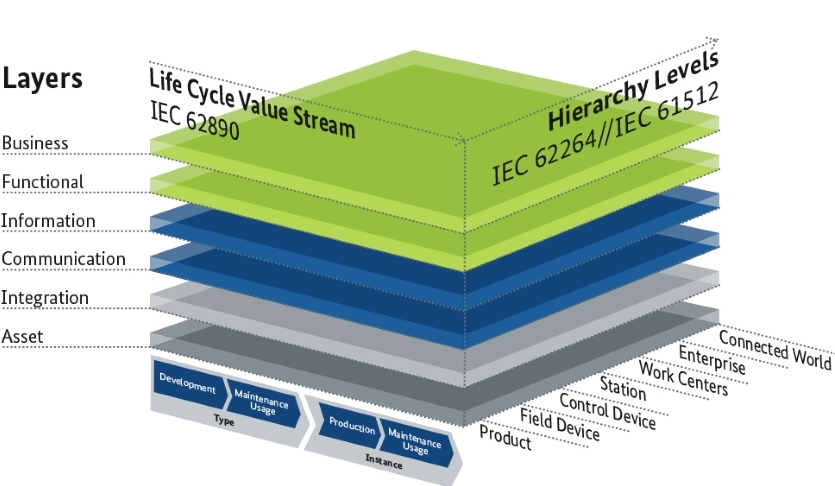
\includegraphics[width=1.0\linewidth]{RAMI.png}
  \caption[Das Referenzarchitekturmodell Industrie 4.0]{Das Referenzarchitekturmodell Industrie 4.0 \citep{BITKOM2015}}
  \label{fig:rami}
\end{figure}

\paragraph{Die Industrie-4.0-Komponente}


\begin{itemize}
  \item Bitkom bzw. Plattform Industrie 4.0 stellt Referenzarchitektur
  \item RAMI bietet die Möglichkeit, Industrie 4.0 UseCases zu verorten, um die für den jeweiligen use case notwendigen Normen und Standards zu identfizieren
  \item horizontale Integration über Wertschöpfungsnetzwerke: Lieferanten, Unternehmen, Produzenten
  \item Durchgängigkeit des Engineerings: Systems Engineering, Modellierung, Simulation
  \item vertikale Integration und vernetzte Pproduktionssysteme mit Echtzeitanforderung
  \item neue soziale Infrastrukturen der Arbeit: Humane-Machine-Systeme und Usability
  \item kontinuierliche Entwicklung von Querschnittssystemen: Netzkommunikation, Breitband, Cloud, Data Analytics, Cyber security
\end{itemize}

(Industrie 4.0 Weltweit)

Das RAMI 4.0 basiert auf den Grundideen des Smart Grids, welches das Stromnetz von der Erzeugung bis zur Verteilung zum Endverbraucher behandelt. Das dreidimensionale Modell kapselt die wichtigsten Funktionalitäten in mehreren Schichten. Dies schafft Flexibilität für die Konzeptionisierung und Realisierung von Industrie 4.0-Lösungen.

\begin{itemize}
  \item Aspekte Industrie 4.0 (Bitkom S. 40) -> Für diese Ziele muss eine Referenz geschaffen werden
  \item 1 - vertikale Integration innerhalb der Fabrik/der Produktion: Vernetzung von Produktionsmitteln wie Automatisierungsgeräte oder Dienste untereinander
  \item 2 - Einbeziehung der Produktes (in meinem Fall produzierte Energie)
  \item durchgängiges Engineering bedeutet: technische, administrative, kommerzielle Daten rund um das Produktionsmittel über Wertschöpfungskette hinweg konsistent halten und jederzeit über das Netzwerk zugreifbar machen
  \item 3 - horizontale Integration über Wertschöpfungsnetzwerke über den Fabrikstandort hinaus und dynamische Bildung von Wertschöpfungsnetzwerken
  \item es gibt RAMI 4.0
  \item und Referenzmodell für die Industrie 4.0-Komponente (s. 45) mit Verwaltungsschale
\end{itemize}







\begin{figure}[h]
  \centering
  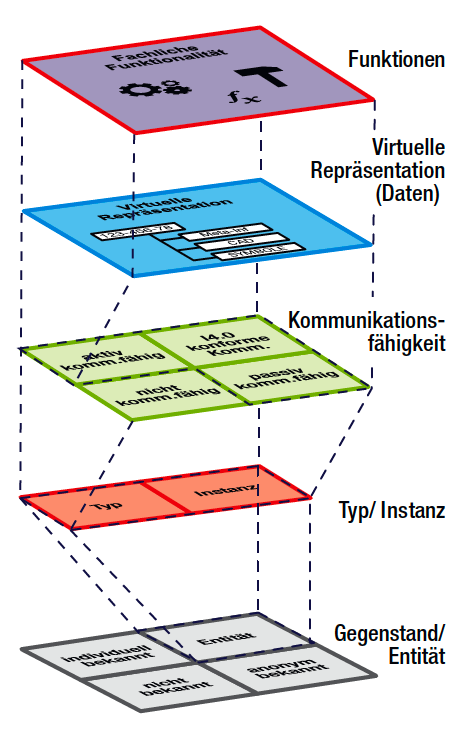
\includegraphics[width=0.5\linewidth]{Ebenen_I40_Kompo.png}
  \caption[Ebenen der Industrie-4.0-Komponente]{Ebenen der Industrie-4.0-Komponente \citep[S. 52]{BITKOM2015}}
  \label{ebenen_i40}
\end{figure}
